\chapter{Versuch 6: Aktiver Tiefpass erster Ordnung}

\section{Einleitung}

In diesem Versuch wird ein aktiver Tiefpass erster Ordnung untersucht. 
Der aktive Tiefpass erster Ordnung besteht aus einem Operationsverstärker
und einem RC-Glied. 
Ziel des Versuchs ist es, die frequenzabhängige Verstärkung eines aktiven
Tiefpasses erster Ordnung zu bestimmen.

\section{Vorbereitung}

\subsection{Benötigte Geräte}

\begin{tabular}[h]{c|c}
    Widerstand 1 k$\Omega$ & 2\\
    \hline
    Widerstand 10 k$\Omega$ & 1\\
    \hline
    Operationsverstärker & \\
    \hline
    Netzgerät & Tenma 72-10495 Digital Control DC Power Supply\\
    \hline
    Funktionsgenerator & T3AFG80\\
    \hline
    Oszilloskop & Keysight DSOX1102A
    \label{tab:Versuch 6: Geräte}
\end{tabular}
\subsection{Schaltungsskizze}

Der Operationsverstärker wird als invertierender
Verstärker verwendet. Die Spannung u\textsubscript{e} wird an den
invertierenden Eingang des Operationsverstärkers angelegt. Die Ausgangsspannung
u\textsubscript{a} wird am Ausgang des Operationsverstärkers abgegriffen.

Die Schaltungsskizze sieht folgendermaßen aus:

\begin{figure}[H]
    \centering
    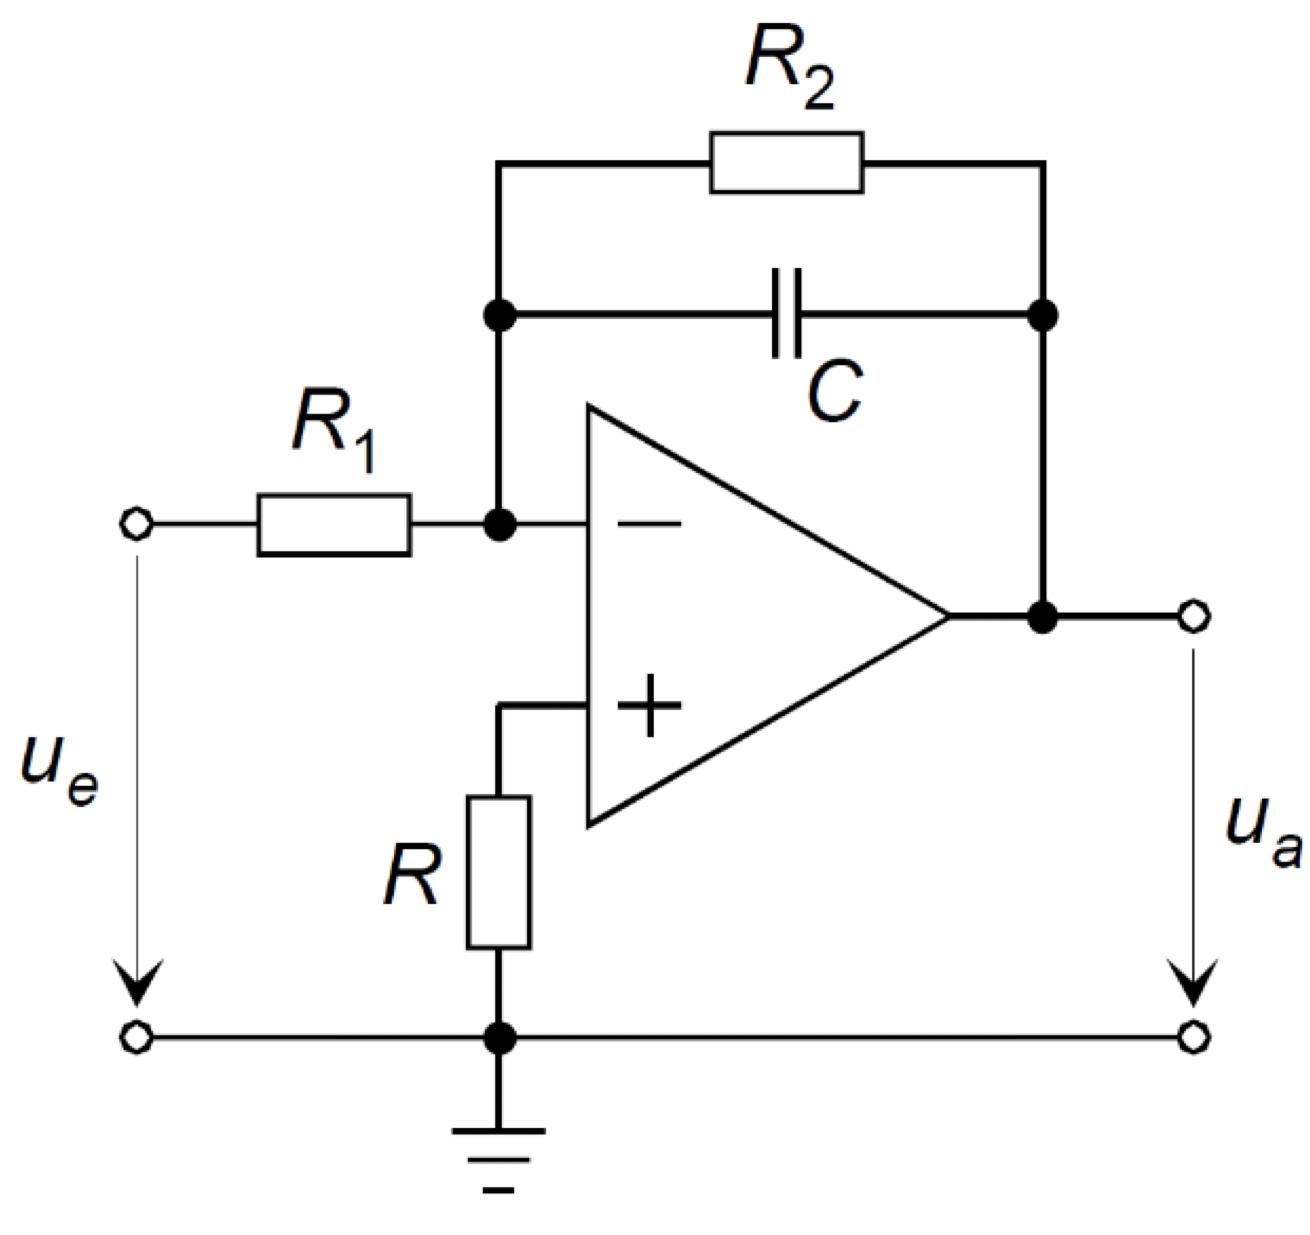
\includegraphics[height=7cm]{images/Versuch6/Schaltungsskizze.jpeg} 
    \caption{Schaltungsskizze}
    \label{fig: Schaltungsskizze}
\end{figure}
Gegebene Größen sind R\textsubscript{1} = 1k$\Omega$,
R\textsubscript{2} = 10k$\Omega$ und C = 10nF.
Des Weiteren ist u\textsubscript{e} als Sinusfunktion mit einer
Amplitude von 15V gegeben.
Zur Berechnung des Widerstands R wird folgende Formel benötigt:

\begin{equation}
    R = R_2|| R_1
    \label{eq:R}
\end{equation}

Als Näherung hierfür wird R\textsubscript{1} eingebaut.

Zur Berechnung der Spannungsverstärkung A\textsubscript{V} als
Funktion der Sinusfrequenz f wird folgende Formel benötigt:

\begin{equation}
    A\textsubscript{V} = -\frac{R_2}{R_1} \cdot \frac{1}{1 + j \cdot 2 \pi \cdot f \cdot R_2 \cdot C}
    \label{eq:AV}
\end{equation}
Messbar ist nur der reele Betrag der Spannungsverstärkung  
$|A\textsubscript{V}| = \sqrt{A\textsubscript{V} \cdot (A\textsubscript{V})^{*}} $.
Im folgenden wird gezeigt, dass es
\begin{equation}
    |A\textsubscript{V}| = C_1\frac{1}{\sqrt{1 + C_2(f)}}
    \label{eq:AV2}
\end{equation} 
gilt. Dafür wird zunächst 
$|A\textsubscript{V}|$ berechnet:

\[
    \begin{aligned}
    |A_V| = \sqrt{\frac{R_2^2}{R_1^2} \cdot \frac{1}{1 + j 2 \pi f R_2 C} \cdot \frac{1}{1 + j 2 \pi f R_2 C}}
    = \frac{R_2}{R_1} \cdot \sqrt{\frac{1}{(1 + j 2 \pi f R_2 C) \cdot (1 + j 2 \pi f R_2 C)}} \\
    = \frac{R_2}{R_1} \cdot \sqrt{\frac{1}{(1 - j 2 \pi f R_2 C + j 2 \pi f R_2 C - j^2 4 \pi^2 f^2 R_2 ^ 2 C^2)}}
    = \frac{R_2}{R_1} \cdot \frac{1}{\sqrt{1 + 4 \pi^2 f^2 R_2 ^ 2 C^2}} \\
    \end{aligned}
\]

Zusammenfassend gilt also:
\begin{equation}
    |A\textsubscript{V}| = \frac{R_2}{R_1} \cdot \frac{1}{\sqrt{1 + 4 \pi^2 f^2 R_2 ^ 2 C^2}}
    \label{eq:AV3}
\end{equation}

Nun werden $C_1$ und $C_2(f)$ aus \ref{eq:AV2} bestimmt: \par
Es gilt für $C_1$ = $\frac{R_2}{R_1}$,
 und für das frequenzabhängige $C_2(f)$ = $4 \pi^2 R_2 ^ 2 C^2$.


\subsection{Schaltungsaufbau}

\section{Versuchsdurchführung}